\documentclass{tmr}

\usepackage{amsmath}
\usepackage[utf8]{inputenc}

\title{Enumeration of Tuples with Hyperplanes} % Avoid extreme use of enumerations (to quote the guidelines of the Monad Reader)
\author{Tillmann Vogt\email{tillk.vogt@googlemail.com}}

\begin{document} 

\begin{introduction}
Have you ever wondered why there are no Enum instances for tuples? If it is possible to assign an integer value to a Bool or a Char then why not to the combination of them? One reason might be that it takes forever to enumerate all 5-tuples of Chars. The other is that the classic method everyone learns at university is letting the digits increase with different speed and makes it unusable for combinatorial problems where you want a quick variation of every digit.  But tuples can also be enumerated so that digits are changing with a fairer distribution, leading to a bunch of problems that I will try to solve in the following.
\end{introduction}

\subsection{ Cartesian product of small sets}

The most straight forward way to  enumerate tuples is to generate all combinations of elements of sets (here finite lists). This is a cartesian product in maths, which can be found in the library haskell-for-maths:
\begin{Verbatim}
cartProd (set:sets) = let cp = cartProd sets in [x:xs | x <- set, xs <- cp]
cartProd [] = [[]]
\end{Verbatim}

For example I recently had to solve a puzzle where I used 

\begin{Verbatim}
cartProd [[0..3],[0..3],[0..3]],
\end{Verbatim}
evaluating to:
\begin{Verbatim}
[[0,0,0],
 [0,0,1],
 [0,0,2],
 [0,0,3],
 [0,1,0],
 [0,1,1], ...].
\end{Verbatim}

This is fine if every combination has to be examined and the sets are small enough. If the sets become too big there is no way to go trough all combinations. This enumeration is problematic for several reasons:
\begin{enumerate}
\item It is not able to enumerate an infinite set at one of its digits.
\item It does not distribute the changes fairly among the digits. The above enumeration is a lexicographic ordering that changes the last digit in the tuple all the time and the first rarely.
\item Every set has to be of the same type, because it is a list.
\end{enumerate}

\subsection{Enumerating $\mathbb{Q} $}
There is another way to enumerate tuples that every computer scientist learns when showing that rational numbers are enumerable. A rational number can be enumerated by giving an axis of natural numbers to each numerator and denominator. Then an enumeration is a path consisting of increasingly longer diagonals (Figure \ref{enum2}).

\begin{figure}[htbp]
  \centering
     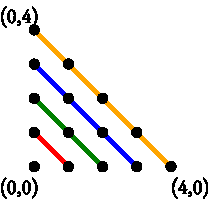
\includegraphics[width=0.2\textwidth]{enum2c.pdf}
  \caption{Enumeration of 2-tuples}
  \label{enum2}
\end{figure}

The next question, that is typically raised in an exercise course, is how to enumerate 3-tuples.
While everybody is thinking hard about a path through 3d-space somebody suggests to use the 2-tuples as a new axis and do the same diagonalization again. This is better than the former solution, because it allows infinite sets in the digits (here $\mathbb{N}$), but there are much more 2-tuples  than single values ($O(x^2)$ against $O(x)$, $x$ being the size of each set at a digit), which again results in an unfair distribution (see the left picture of Figure \ref{enum3} that shows the path that is biased towards one axis). Doing this repeatedly results in distributions where one digit grows with $O(x^3)$ for 4-tuples, $O(x^4)$ for 5-tuples.

This unfairness can be avoided in 4-tuples, generally $2^n$-tuples, and at least be made less severe by choosing tuples for both axes, but it leaves the non-$2^n$-tuples still with an unfair distribution.

\subsection{Diagonals are Hyperplanes}
If you look again at the diagonals of the enumeration of 2-tuples then you can observe that a diagonal (\eg $ [ (0,4), (1,3), (2,2), (3,1), (4,0) ])$ always consists of tuples whose sum of digits is constant:
$  [ (x,y)  \mid  x+y  = c ], c \in \mathbb{N}. $
The same idea can be applied to 3-tuples. The right picture of Figure \ref{enum3} is an enumeration path where the sum of the digits stay constant for an enumeration plane:
\[  [ (x,y,z)  \mid  x+y+z  = c ], c \in \mathbb{N}. \]

It is obvious that this enumeration generates tuples with a fair distribution of changes in the digits. Like the 2d-case It is also is a repeated generation of hyperplanes. A hyperplane is a $(n-1)$-dimensional subset of a $n$-dimensional space that divides the space in two, \eg  a diagonal line in 2d-space or a plane in 3d-space.

\begin{figure}[htbp]
  \centering
    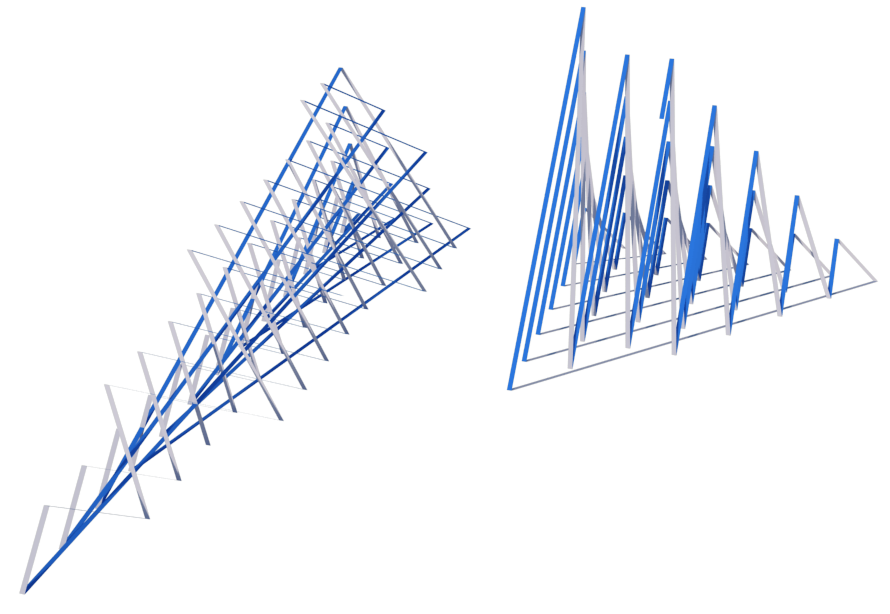
\includegraphics[width=\textwidth]{enumerate2.png}
  \caption{Enumeration with repeated diagonalization (left), with hyperplanes (right)}
  \label{enum3}
\end{figure}

\section { Enum Instances}
Haskell uses typeclasses to enumerate values. This is a very nice feature because it permits to nest arbitrary tuples and values whose type have an \verb|Enum| instance. Take for example the \verb|Enum| instance for 2-tuples:

\begin{Verbatim}
instance (Enum a, Enum b, Eq a, Eq b, Bounded a, Bounded b)
                    => Enum (a, b) where
\end{Verbatim}
If \verb|a| is enumerable and \verb|b| is enumerable then the tuple \verb|(a,b)| is also enumerable. Because the values are enumerated from the low boundary to the high boundary and comparisons have to be made, \verb|a| and \verb|b| are also in \verb|Eq| and \verb|Bounded|.
The goal is now to be able to write
\begin{Verbatim}
( enumFrom (0,(1,2),3) ) :: [(Word8,(Word8,Word8),Word8)]
\end{Verbatim}
This is an example for an arbitrary nesting, with arbitrary starting values, that evaluates to (you will see later why):
\begin{Verbatim}
[(0,(1,2),3), (0,(2,1),4), (0,(3,0),5), ...]
\end{Verbatim}


A type that should be enumerable can be made an instance of the \verb|Enum| typeclass by defining at least two functions:
\begin{Verbatim}
    toEnum           :: Int -> a
\end{Verbatim}
which returns a value of type \verb|a| to a number and
\begin{Verbatim}
    fromEnum         :: a -> Int
\end{Verbatim}
which returns a number to a value of type \verb|a|. There exist instances for primitive types like Char, Bool and Int (duh). 
The following functions are defined with \verb|toEnum| and \verb|fromEnum|, but can be overridden:

\begin{Verbatim}
    succ, pred       :: a -> a
    enumFrom         :: a -> [a]             -- [n..]
    enumFromThen     :: a -> a -> [a]        -- [n,n'..]
    enumFromTo       :: a -> a -> [a]        -- [n..m]
    enumFromThenTo   :: a -> a -> a -> [a]   -- [n,n'..m]
\end{Verbatim}

In our case we will overwrite \verb|succ| (the successor in the enumeration) and \verb|pred| (the predecessor), because they can be calculated faster than using something like
\begin{Verbatim}
succ = toEnum . (`plusInt` oneInt)  . fromEnum
\end{Verbatim}

\section{succ, pred}
The whole idea of this enumeration started with functions that matched tuples with certain patterns and produced new tuples. Changes happen when a 0 is reached in the tuple. Because enumeration of arbitrary types should be possible, 0 is replaced by minBound. Instead of looking at a tuple it is faster to look only at the important digits:
\small
\begin{Verbatim}
succ (a,b,c) =
 if c == minBound then
  if b == minBound then
   if a == minBound then (succ a  , b       , c      ) -- (a,b,c) was (0,0,0)
                    else (pred a  , succ b  , c      ) --   (b,c) was   (0,0)
                   else  ( a      , pred b  , succ c ) --      c  was      0
                 else
 if b == minBound then -- switching to the next hyperplane
 if a == minBound then (toEnum (fc+1), minBound, minBound)--(a,b,c) was (0,0,c)
                  else (pred a  , toEnum (fc+1), minBound)--  (b,c) was   (0,c)
                  else (a       , pred b       , succ c ) -- generating diagonals
  where
    fc = fromEnum c
\end{Verbatim}
The last tuple generates diagonals and every \verb|else| in the first half of this code generates a higher dimensional hyperplane.
The line \verb|(toEnum (fc+1), minBound, minBound)| makes a switch to a new hyperplane, that is one bigger in the sum of digits than the last hyperplane. Because the types in the tuple can be different from each other \verb|fromEnum c| and \verb|toEnum (fc+1)| have to be used instead of \verb|succ| and \verb|pred|. The function \verb|pred| for 3-tuples is implemented similarly:

\begin{Verbatim}
  pred (x,y,z) =
   if z == minBound then
    if y == minBound then
     if x == minBound then error "Enum.pred{(x,y,z)}: tried to take `pred' of minBound"
                      else (minBound, minBound, toEnum (fx-1)) -- (fy,fz) was (0,0)
                     else  (succ x  , minBound, toEnum (fy-1)) --     fz  was    0
                    else   (x       , succ y  , pred z       )
    where
      fx = fromEnum x
      fy = fromEnum y
\end{Verbatim}
Here the line \verb|(minBound, minBound, toEnum (fx-1))| makes a switch to a lower hyperplane.

\subsection{Avoiding some typewriting}

The function \verb|succ| could be defined for the other tuples in the same way, but this is a lot of typing for 15-tuples (the biggest tuple that is allowed). 
There is a pattern in the tuple that is produced when a certain pattern of zero or non-zero values in an inbound tuple occurs.
One can come up with functions that do the same as the upper \verb|succ| function when seeing an $n$-tuple as a list.
But a tuple can have all kinds of types and therefore is not compatible with an ordinary list. What to use? A heterogeneous list? One can also use a trick that transforms a tuple into a finite list-like structure and back:

\begin{Verbatim}
to5Tuple  ((((a,b),c),d),e)  = (a,b,c,d,e)
\end{Verbatim}

Then \verb|succ| can be defined like this:
\begin{Verbatim}
succ fz s ((x,y),z)
 | y /= minBound && z == minBound= ((x, pred y), succ z)
 | y == minBound && z == minBound=  (succ fz False (x,y), z)
 | y /= minBound && z /= minBound=((x,pred y), if s then succ z else toEnum (fz+1))
 | y == minBound && z /= minBound=  (succ fz False (x,toEnum fz), minBound)
\end{Verbatim}
Here \verb|y| and \verb|z| should be imagined as single values while \verb|x| can be the list-like structure. 
Unfortunately the upper code gives a type error in Haskell (Occurs check: cannot construct the infinite type: t0 = (t0, a0)), which is understandable because the compiler can't know that this nesting terminates without a termination analyzer. In the expression \verb|((a,b),c)|  \verb|a| cannot stand for another tuple \eg \verb|(((d,e),b),c)| and the compiler does not know that we are not constructing an infinite type.
So we just define \verb|succ| for all tuples, like this:

%\textit{% This is a comment}
%\textcolor{red}{Third}

\begin{Verbatim}[commandchars=\\\{\}]
\fbox{succ5} :: ( Enum a, Enum b, Enum c, Eq a, Eq b, Eq c,
           Bounded a, Bounded b, Bounded c) =>
         Int -> Bool -> ((\fbox{((a,b),c)},d),e) -> ((\fbox{((a,b),c)},d),e)
\fbox{succ5} fz s ((x,y),z)
| y /= minBound && z == minBound = ((x, pred y), succ z)
| y == minBound && z == minBound =  (\fbox{succ4} fz False (x,y), z)
| y /= minBound && z /= minBound =((x,pred y), if s then succ z else toEnum (fz+1))
| y == minBound && z /= minBound =  (\fbox{succ4} fz False (x,toEnum fz), minBound)
\end{Verbatim}
To define the other \verb|succ| functions one only has to change the number after the two \verb|succ|-functions in the body accordingly. 

I haven't found an easy way to do the same with \verb|pred|, because the last value in the tuple depends on values at various positions.
%This would become completely unusable if the cases for \verb|maxBound| (see next section) were introduced in there. %\ref{boundaries}).

\subsection{Reaching boundaries}
Until now only tuples with big sets were enumerated. The fair enumeration guaranteed that no boundaries were reached. But if tuples with Bools are enumerated, the boundary is reached fast. Looking at an enumeration of 3-tuples of Word8s it can be seen that some boundaries have to be crossed, to get at an exhaustive enumeration:

\begin{Verbatim}
> enumFrom (0,0,0) :: [(Word8,Word8,Word8)]  -- Word8 is used because it starts at 0
\end{Verbatim}

evaluates to:

\begin{Verbatim}
[(0,0,0),(1,0,0),(0,1,0),(0,0,1),
 (2,0,0),(1,1,0),(1,0,1),(0,2,0),(0,1,1),(0,0,2),
 (3,0,0),(2,1,0),(2,0,1),(1,2,0),(1,1,1),...]
\end{Verbatim}
Replacing \verb|0,1| with \verb|False,True| the upper list contains all combinations of \verb|(Bool,Bool,Bool)|, but also intermediate steps:
\begin{Verbatim}
[(False,False,False),(True,False,False),(False,True,False),(False,False,True),
 (2,False,False),(True,True,False),(True,False,True),(False,2,False),(False,True,True),
(False,False,2), (3,False,False),(2,True,False),(2,False,True),(True,2,False),
(True,True,True)]
\end{Verbatim}

To allow values that cross boundaries we introduce a data type that consists of a normal value or an integer:
\begin{Verbatim}
data J a = Jst a | I Int
\end{Verbatim}
Because we enumerate only in ascending order from some value, we only have to implement cases where the upper boundaries are crossed and luckily the \verb|succ| functions are not so big:

\begin{Verbatim}
succ5 :: ( Enum a, Enum b, Enum c, Enum d,Enum e, Eq a, Eq b, Eq c, Eq d, Eq e,
           Bounded a, Bounded b, Bounded c, Bounded d, Bounded e) =>
         Int -> Bool -> ((((J a,J b),J c),J d),J e) -> ((((J a,J b),J c),J d),J e)
succ5 fz start ((x,y),z)
  | not (minB y) && (minB z) = ((x, (pre y)), suc z)
  |     (minB y) && (minB z) = (succ4 fz False (x,y), z)
  | not (minB y) && not (minB z) = ((x, (pre y)), if start then suc z else v (fz+1) z)
  | (minB y) && not (minB z) = (succ4 fz False (x, v fz z), Jst minBound)
\end{Verbatim}
Helper functions like \verb|suc|, \verb|pre| and \verb|v| take care of the stepping over boundaries.

\section { The size of enumeration hyperplanes }

The sizes of enumeration hyperplanes are needed to assign a tuple to a number (\verb|toEnum|) or to find the place of a tuple in an enumeration  (\verb|fromEnum|).  From the right picture of Figure \ref{enum3} it can be seen that the 2d-hyperplanes consist of 1d-hyperplanes (diagonals).  Generally an $n$-dimensional space is enumerated with (n-1)-dimensional hyperplanes. These hyperplanes are again enumerated by (n-2)-dimensional hyperplanes (and so on). The size of an $n$-dimensional enumeration hyperplane can be deduced by looking at the two and three dimensional case.

The size of our 2d-hyperplane (a plane of diagonals) is a well known problem that Gauß solved at the age of 9:

\begin{equation}\label{gauss}
 1+2+3+4+5 ... + n  = \sum_{k=1}^{n} k =  n (n+1)/2
\end{equation}

A 3d-enum-hyperplane consists of increasingly bigger 2d-enum-hyperplanes:

\begin{equation} \label{poly3d}
\begin{split}
& 1 +\\
&(1+2) +\\
&(1+2+3) + ... \\
& = \sum_{k=1}^{n}  k (k+1)/2 \\
& = \sum_{k=1}^{n} (\frac{k}{2} + \frac{k^2}{2}) = \frac{ n (n+1) }{2*2} + \frac{2n^3+3n^2+n}{6*2} 
\end{split}
\end{equation}

In (\ref{poly3d}) we sum over the polynomial of the Gauß sum (\ref{gauss}).

To calculate the sum of $k^2$'s the Bernoulli formula for sums of powers is used:

\begin{equation} \label{bernoulli}
\boxed{
\sum_{k=1}^{n-1} k^p = \frac{1}{p+1} \sum_{j=0}^{p} \binom{p+1}{j} \beta_{j} n^{p+1-j}
}
\end{equation}



Applying this pattern again, leads to the size of a 4d-hyperplane :

\begin{equation}\label{poly4d}
\begin{split}
 & 1 +\\
 &(1+(1+2) )+ \\
 &(1+(1+2)+(1+2+3)) + ... = \sum_{k=1}^{n} (\frac{ k (k+1) }{2*2}  + \frac{2k^3+3k^2+k}{6*2})
\end{split}
\end{equation}

\subsection { Calculating it }

The last section showed that the size of a hyperplane can be given with a polynomial. The common way to represent a polynomial is to only use its coefficients. Therefore a function is needed to evaluate a polynomial in $n$:
\small
\begin{Verbatim}
       polynomial :: Int -> [Rational] -> Rational
       polynomial n coeffs = foldr (+) 0 (zipWith nPowerP coeffs [1..])
         where nPowerP a_j p = a_j * (fromIntegral (n^p))
\end{Verbatim}

The coefficients of a polynomial in $n$ that results from $\sum_{k=1}^{n-1} k^p$ are needed. At position $n^{p+1-j}$ this is:

\begin{equation} \label{bernoulli}
coefficient(j) = \frac{1}{p+1} \binom{p+1}{j} \beta_{j}.
\end{equation}

The combinat-library that can be found on hackage provides some parts of the Bernoulli formula: The Bernoulli numbers $\beta_{j}$ and the binomial coefficient. With that a part of the Bernoulli formula can be implemented by

\small
\begin{Verbatim}
sumOfPowers :: Int -> [Rational]
sumOfPowers p = reverse [ (bin j) * (ber j) / ((fromIntegral p)+1) | j <- [0..p] ]
  where bin j = fromIntegral (binomial (p+1) j)
        ber j | j == 1 = negate (bernoulli j) -- see wikipedia entry
              | otherwise = bernoulli j
\end{Verbatim}

Because of $-j$ in $n^{p+1-j}$ \verb|reverse| is needed.
We apply this formula to a polynomial with increasing degree, first $k$, then $\frac{k}{2} + \frac{k^2}{2}$, ....

The size of an n-dimensional hyperplane can be calculated by repeatedly applying the Bernoulli formula (\verb|map sumOfPowers|) to the $n^p$ after the coefficients of a polynomial, and adding the coefficients (\verb|merge|):

\small
\begin{Verbatim}
hyperplaneSize :: Int -> Int -> Int
hyperplaneSize dim n = round (genPolynom 1 [1])
  where genPolynom :: Int -> [Rational] -> Rational
        genPolynom d coeffs | d == dim  = polynomial n coeffs
                            | otherwise = genPolynom (d+1)
                              (merge coeffs (map sumOfPowers [1..(length coeffs)]))

merge coeffs ls = foldr myZip [] multiplied_ls
  where multiplied_ls = zipWith (\c l -> map (c*) l) coeffs ls
        myZip (l0:l0s) (l1:l1s) = (l0+l1) : (myZip l0s l1s)
        myZip a b = a ++ b
\end{Verbatim}

\subsection {fromEnum }
In the last section we saw how to calculate the size  of the $n-th$ enumeration hyperplane of a $d$-dimensional space. To calculate \verb|fromEnum| lists of these sizes are used and an increasingly bigger sum of hyperplanes:

\begin{Verbatim}
ssizes d = [ sum (take n sizes) | n <- [1..] ]
  where sizes = [ hyperplaneSize d i | i <- [0..] ]

summedSizes :: Int -> Int -> Int
summedSizes dim n = (ssizes dim) !! n
\end{Verbatim}
The function \verb|fromEnum| takes a tuple and gives back an integer. Using \verb|fromEnum| at every digit of the tuple, the tuple itself contains integers and a general function \verb|fe| can be used that transforms a list of integers into a single integer:

\begin{Verbatim}
  fromEnum (a,b,c,d) = fe [fromEnum a, fromEnum b, fromEnum c, fromEnum d]
\end{Verbatim}

As defined in the beginning a hyperplane consists of all tuples whose sum of digits is constant. To calculate the position inside the hyperplane, the hyperplane is projected on dimension lower. This can be imagined by the plane in 3d that is projected to 2d by setting one coordinate to zero. There are two ways to do this in 2d, three ways in 3d, generally n ways in an n-dimensional space. This is a degree of freedom that can be exploited further to influence how fast values change (inside a hyperplane!).
For the upper 4-tuple we always set the first value to zero and have to calculate therefore (\verb|a1| being \verb|fromEnum a| and so on):

\begin{Verbatim}
 (summedSizes 3    (a1+b1+c1+d1) ) +
 (summedSizes 2       (b1+c1+d1) ) +
 (summedSizes 1          (c1+d1) ) +
                             d1
\end{Verbatim}

For all dimensions (\eg the 11 dimensions in string theory):
\begin{Verbatim}
fe [x] = x
fe (x:xs) = ( summedSizes (length xs) (foldr (+) 0 (x:xs)) ) + (fe xs)
\end{Verbatim}

\subsection {toEnum }
To calculate \verb|toEnum| we have to invert the upper process. Lets look again at the example of a 4-tuple. To get \verb|a1| it is enough to know the two sums \verb|(a1+b1+c1+d1)| and \verb|(b1+c1+d1)| and calculate the difference:

\begin{Verbatim}
differences :: [Int] -> [Int]
differences [x] = [x]
differences (x:y:ys) = (x-y) : (differences (y:ys))
\end{Verbatim}

If \verb|toEnum| gets the argument \verb|n| and the tuple has dimension d then we search where n is located between the sums of hyperplanes, remember this number (\verb|planes|), subtract the size of the smaller hyperplane and do the same again with the rest but one dimension below:

\begin{Verbatim}
te :: Int -> Int -> [Int]
te dim n = differences $ reverse $ fst $ foldr hplanes ([],n) [1..dim]

hplanes :: Int -> ([Int],Int) -> ([Int],Int)
hplanes d (planes,rest) = ((fst hp):planes, snd hp)
  where hp = (hyperplane d rest)

hyperplane dim n = ( (length filtered) - 1, n - (if null filtered then 0 else last filtered) )
  where filtered = filterAndStop [ summedSizes (dim-1) i | i <- [0..] ]
        filterAndStop (x:xs) | x <= n     = x : (filterAndStop xs)
                             | otherwise = []
\end{Verbatim}

\section{Previous work and Conclusion}
The idea to enumerate tuples like this is a year old. While writing \verb|Enum|-Instances it seemed interesting enough to write an article about it. So far I could not find a reference mentioning it (\eg Donald Knuth: Generating All Tuples and Permutations). I think it can save some time in combinatorial problems or when one has to chose an option among several possibilities, \eg in generating a user interface.

\subsection{Code to generate the images}

The images were generated with collada-output and diagrams.

\begin{verbatim}
main = B.writeFile "test.svg" $ toLazyByteString $
                renderDia SVG (SVGOptions (Dims 100 100)) (enum2 ||| enum3)

-- 2d enumeration

enum2 =  ((stroke ( mconcat $ translatedPoints)) # fc black # fillRule EvenOdd )
      <> enumLines
      <> ( translate (-1,-1) $ text' "(0,0)")
      <> ( translate (4 ,-1) $ text' "(4,0)")
      <> ( translate (-1, 4.25) $ text' "(0,4)")

translatedPoints = map (\v -> translate v (circle 0.15) ) points

points = map (\(x,y) -> (fromIntegral x, fromIntegral y))
                              $ take 15 ( all2s :: [(Word8,Word8)] )

enumLines = mconcat $ colorize (map enumLine (pointList points []) # lw 0.1)
 where enumLine l = fromVertices (map P l)
       pointList []         l = [l]
       pointList ((0,y):ps) l = ((0,y):l) : ( pointList ps [] )
       pointList ((x,y):ps) l = pointList ps (l ++ [(x,y)])

colorize = zipWith (\c d -> d # lc c) [yellow,red,green,blue,orange]

text' t = stroke (textSVG t 0.8) # fc black # fillRule EvenOdd
\end{verbatim}

\end{document}
